%=================================================================
\section{Introduction}\label{sec-intro}


%\todo{Narrow down to a topic; Dig a hole; Fill the hole}
%\todo{Formula for Introduction}

%\gangli{``narrow in on topic'' reminds you 
%that readers and reviewers only know that this is a AI or HTM research paper (and maybe have read the title/abstract). 
%You need to help them figure out what topic and area of research paper this is. 
%You _don't_ need to wax poetic about the topic's importance.}

%\gangli{`dig a hole'' reminds you that 
%you need to convince the reader that there's a problem with the state of the world. 
%Prior work may exist but it's either missing something important or there's a missing opportunity. 
%The reader should be drooling for a bright future just out of reach.}

%\gangli{``fill the hole'' reminds you to show the reader 
%how and why the paper they're reading will fix these problems and deliver us into a better place. 
%You don't need a whirlwind summary of the technical details, 
%but you need readers convinced (and in a good mood) to keep reading.}

%\gangli{A good paper introduction is fairly formulaic. 
%If you follow a simple set of rules, 
%%you can write a very good introduction. 
%The following outline can be varied. 
%For example, 
%%you can use two paragraphs instead of one, 
%or you can place more emphasis on one aspect of the intro than another. 
%But in all cases, 
%all of the points below need to be covered in an introduction, 
%and in most papers, 
%you don't need to cover anything more in an introduction.}


%\todo{The importance of the area}
%\blindtext
%\todo{Motivation}
Air pollution is significant problem which arises due to many reasons.
Among them technological evolution takes high priority.
However, people need to move on with the technical world 
while keeping sustainable environment for the future generation.
For that, almost all industrialization production processes need 
to concern on their emissions into the environment.
For example, many industries tend to left different types of air 
particles into the atmosphere as a result of their production process.
Though it does not seems to have quick threat on environment and the human life,
it has long life impact. Consequently, people tend to find the solutions to 
mitigate these pollution in order to enhance the best balance between 
the industrialization and the environment protection. 
Initially, data is the major asset for everything in the world.
Because, every application had data driven structure to analyse the current trends 
in order to predict the future impacts or enhancements.
Machine learning and Artificial intelligent play vital role in the data driven applications. 
Therefore, in such studies present prediction and detection models based on the existing data.

%\todo{The problems faced by most current methods}
%\blindtext
%\todo{What is the specific problem considered in this paper?}
In this study we reveals the high performing prediction model
using supervised learning model called regression, to predict the air pollution.
For that, we use temperature values, relative and absolute humidity, 
and 5 sensor values as predictor variable for several months.
The given target variables are compositions of carbon monoxide, benzene, and nitros oxide.

%\todo{What can be addressed by existing methods; Why those problems are challenges to existing methods?}
%\blindtext
\todo{Contribution}
In this paper we show that the model prediction behavior on multicollinearity based predictor variables. 
Since this is a labeled dataset, we 
decide to perform supervised learning on training data to propose a model.
Moreover, prepossessing helps to determine the 
correlations between the different features.
This predictor variables indicate multicollinearity.
Due to that, It is impossible to propose a linear correlation based model for this scenario. 
Therefore, we decide to continue our empirical 
results using the multi correlation based regression method called rigid regression. 
Our main contribution is as follows,
\begin{itemize}
	\item First we analyse, how much of multicollinarity consists among the given predictor variable using heatmap visualization.
	\item Second we show how target air pollution components behave over certain period.
	\item Third we clearly show predicted results by using the proposed regression model.
\end{itemize}

\begin{figure}
  \centering
  \selectcolormodel{rgb}
 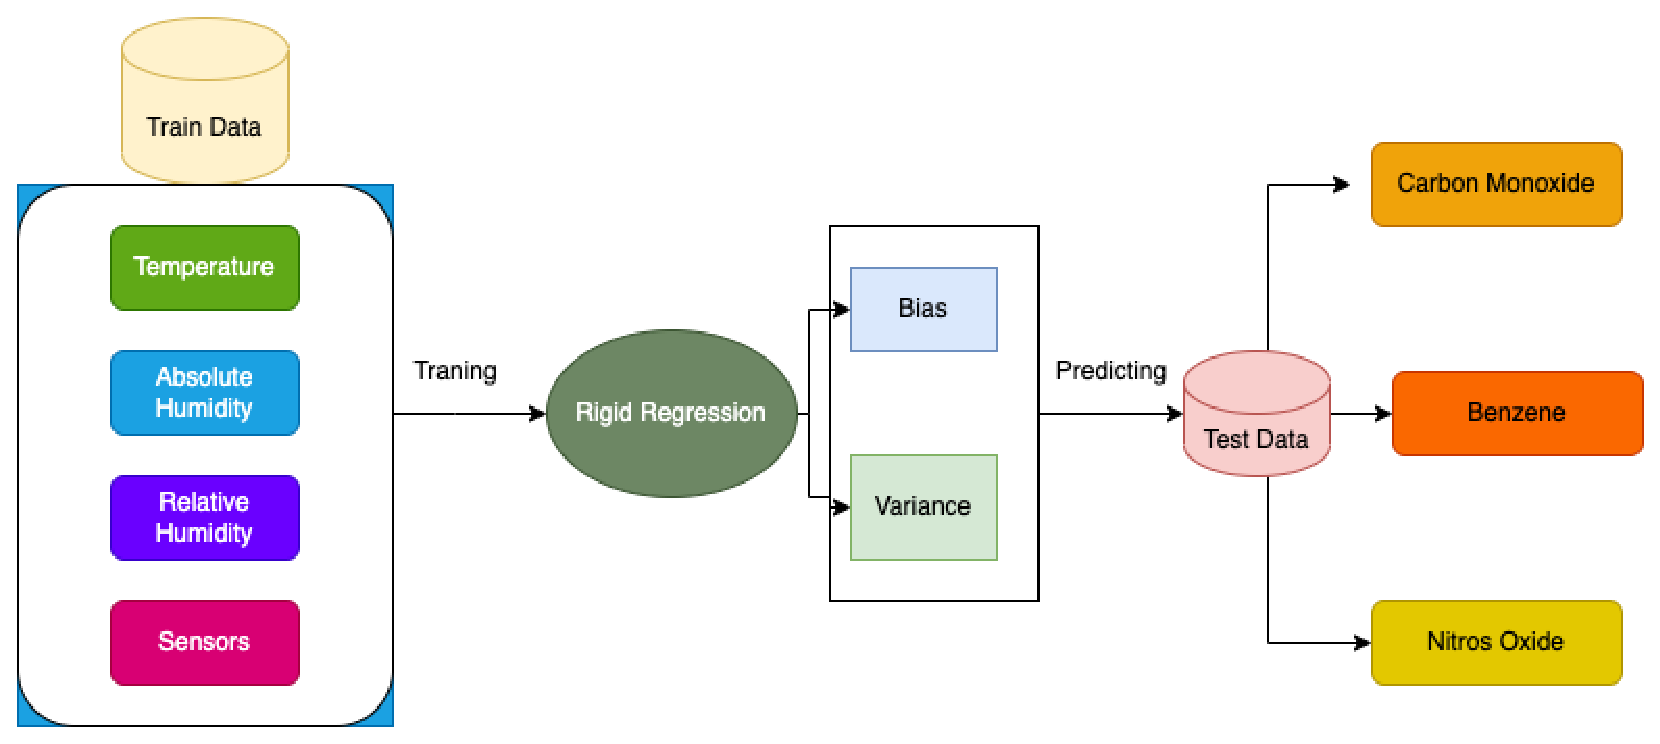
\includegraphics[width=1.0\linewidth,height=0.6\linewidth]{graphics//Fig_AirPrediction.eps}
  \caption{Proposed Framework} \
  {image1:Fig_AirPrediction}
  %label{Fig_AirPrediction}
\end{figure}

%\todo{What provides the motivation of this work? What are the research issues? What is the rationale of this work? }
%\blindtext
%\todo{At a high level what are the differences in what you are doing, and what others have done? }
Most of the other studies try to reveal prediction models without considering multicollinarity. 
However, the importane of our method is addressing multicollinarity in high level.
%\todo{What we have done and what are the contributions.}
%\blindtext
%\todo{A roadmap for the rest of the paper}
The rest of this paper is structured as follows:
Section 2 describes the preliminary studies that we conducted before proposing this model.
The method of this proposed model is in Section 3.
Section 4 discusses the empirical findings of the study presenting performance comparison
and Section 5 involves discussion and 6 elaborate on future directions conclusions.


%\gangli{A few general tips:
%Don't spend a lot of time into the introduction 
%telling the reader about what you don't do in the paper. 
%Be clear about what you do do.
%Does each paragraph have a theme sentence that sets the stage for the entire paragraph? Are %the sentences and topics in the paragraph all related to each other?}

%\gangli{Does each paragraph have a theme 
%sentence that sets the stage for the entire paragraph? 
%Are the sentences and topics in the paragraph all related to each other?}

%\gangli{Do all of your tenses match up in a paragraph?}


%This is for~\cref{tbl:overall-experiments}, 
%\todo[fancyline]{Testing.}
%and this is for~\cref{sec-conclusions}.
%\todo[noline]{A note with no line back to the text.}%
%\gangli{This is comment from Gang.}
%\qwu{Response from QW}

%\missingfigure[figcolor=white]{Testing figcolor}

%\begin{ConferenceOnly}
%We have \SI{10}{\hertz},
%\si{\kilogram\metre\per\second},
%the range: \SIrange{10}{100}{\hertz}.
%$\nicefrac[]{1}{2}$.

%\missingfigure{Make a sketch of the structure of a trebuchet.}

%\end{ConferenceOnly}


%For~\cref{eq:test},
%as shown below:

%\begin{equation}\label{eq:test}
%a = b \times \sqrt{ab}
%\end{equation}

%\blindmathpaper

\section{Preliminaries} \label{sec-preliminaries}

Initially, regression problems 
anayse the correlation between 
the predictor variable and the response variables~\citep{uyanik2013study}.
Most probably, regression problems define correlation 
between two quantitative variables.
This is indicate as linear regression if it represents 
relationship by straight line. 
However, logistic regression and non-linear regression show curve shape relationship. 
Moreover, the challenge is 
selecting appropriate predictor 
variable for the given response variable. 
In this scenario we have three 
response variables such as 
carbon monoxide, benzene and notrous oxide compositions.

\begin{figure}
  \centering
  \selectcolormodel{rgb}
 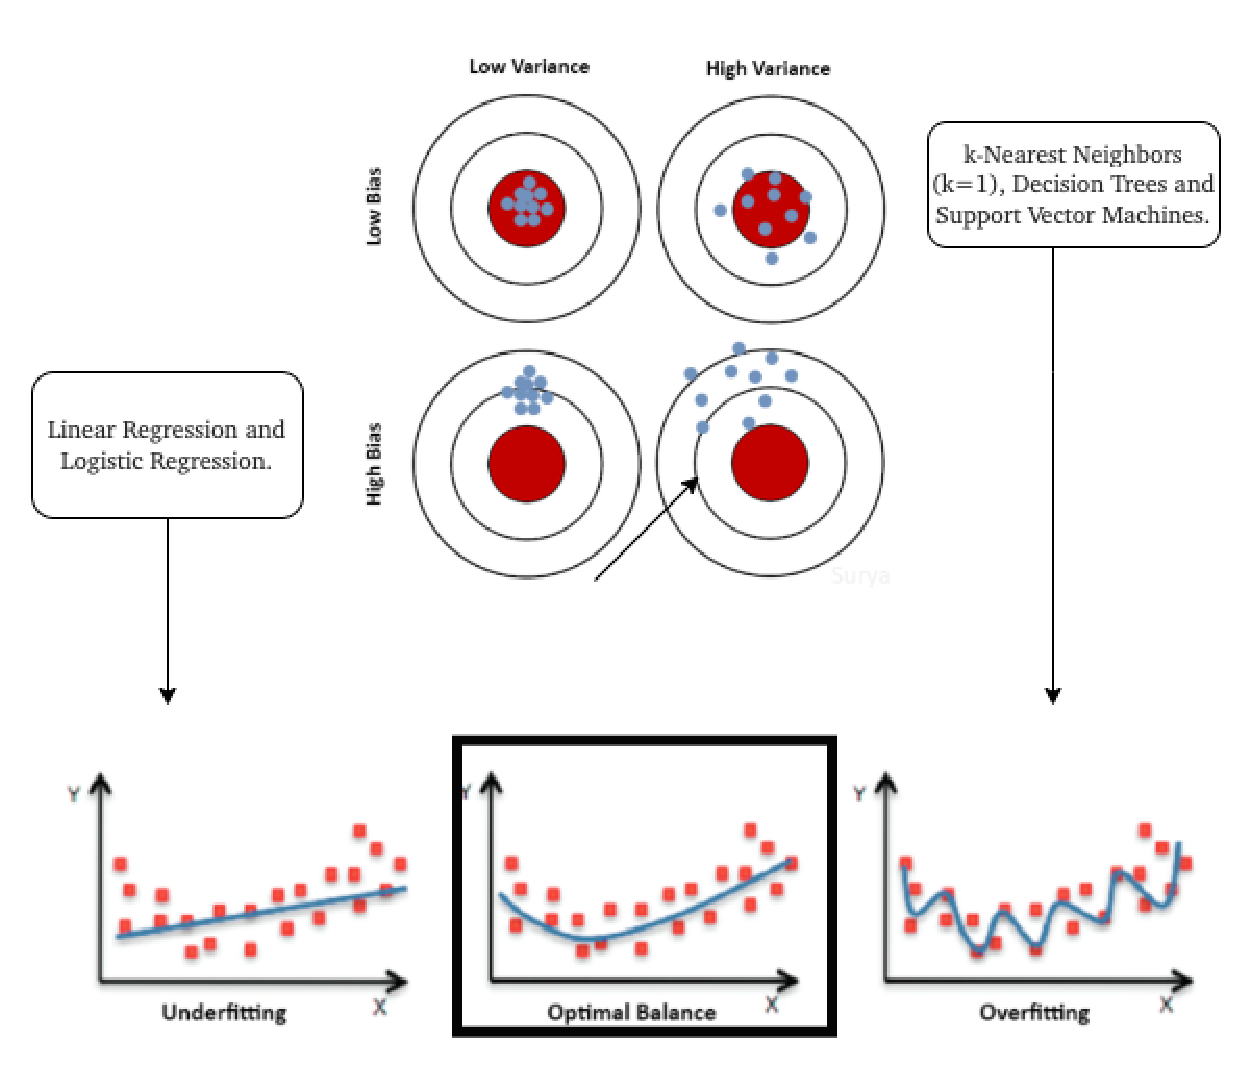
\includegraphics[width=0.8\linewidth,height=0.7\linewidth]{graphics//Bias_and_VrarianceAll.eps}
  \caption{Bias and Variance for Prediction Accuracy} \label{Bias_and_VrarianceAl}
\end{figure}

However, when there is more predictors available in training set it is obvious to have correlation among predictors. 
In such cases, we cannot use linear regression methods to 
derive prediction models only using two predictors.
Because, Once we select one predictor variable to derive 
correlations between that 
selected predictor and the given response variable, we need to 
assume other predictors have no or less impact on that correlation.
Depending on different factors such as experience, historical 
data one response may be affected by more predictors~\cite{seber2012linear}. 
In this study we are working on same kind of scenario.

Machine learning allows machines to analyse existing data and 
predict on them. These predictions comes as the 
artificial intelligent models which can outperform on future data predictions. 
However, making prediction cannot be always trustworthy 
to have $100\%$ accuracy. 
Therefore, it allows to have predictions errors. 
These errors are called Bias and Variance.
We use this bias and variance values in the models to state 
accuracy levels of proposed models in our evaluation process.
Bias is a training data error while variance is the testing data error.
As in the Figure~\cref{Fig_BiasVariance}, we can have four types of error levels.
However, low bias and low variance models are the bet fitted models.
Because the both training and testing data fitted exactly on
the model as in optimal balance graph.
However, since it is impossible to derive non-error research
work target to derive low bias, high variance models such as
decision tree, support vector machines and k-nearest neighbour or high bias, low variance methods such as regression models.
In this study we uses regression models and we prove that
we are achieving underfittiing scenarios as illustrated in Figure \cref{Bias_and_VrarianceAll}
In linear regression, we normally derive a best fitted line to represent all training data set.
However, due to the multiple core relations among predictors, we uses rigid regression in which uses penalty term to 
augment the loss function of the linear regression for better performance.

\gliMarker  %TODO: GLi Here

\section{Method} \label{sec-method}

\subsection{Prepossessing and Multicollinearity}

\begin{figure}
  \selectcolormodel{rgb}
  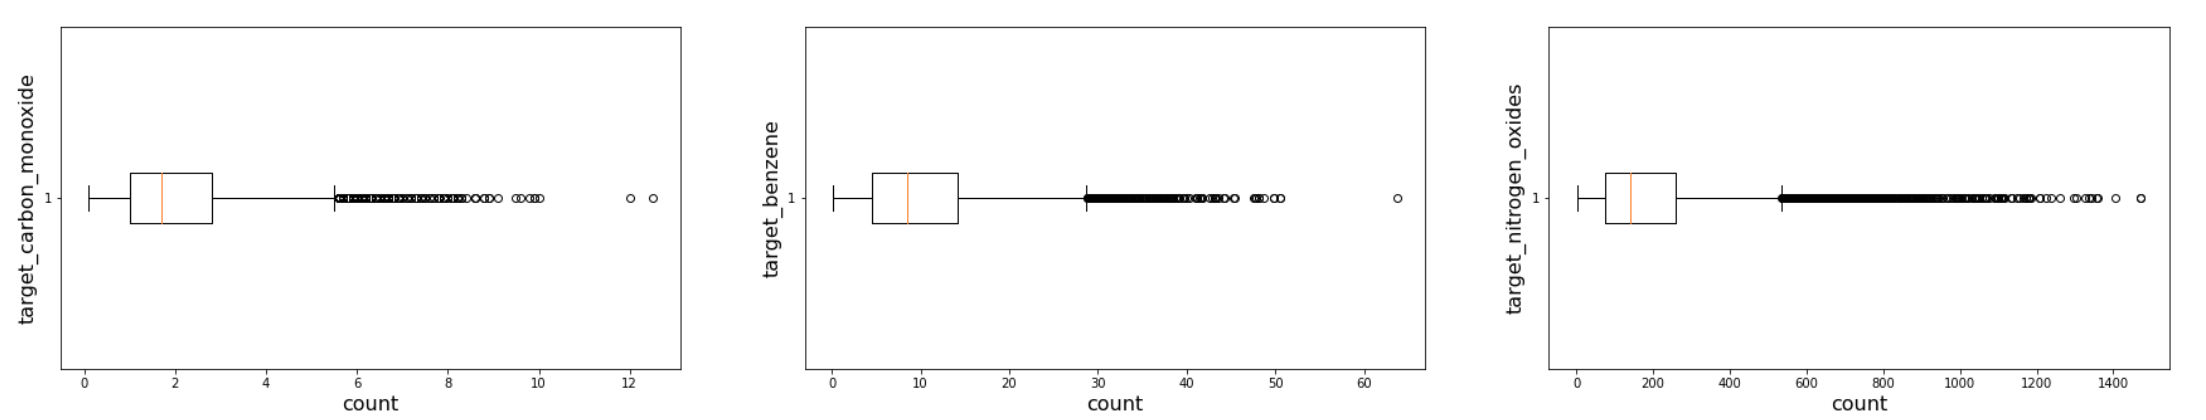
\includegraphics[width=1.0\linewidth,height=0.4\linewidth]{graphics//Fig_Boxplot.eps}
  \caption{Response data distribution and Outlier Detection.} \label{Fig_Boxplot}
\end{figure}

\begin{figure}
  \centering
  \selectcolormodel{rgb}
 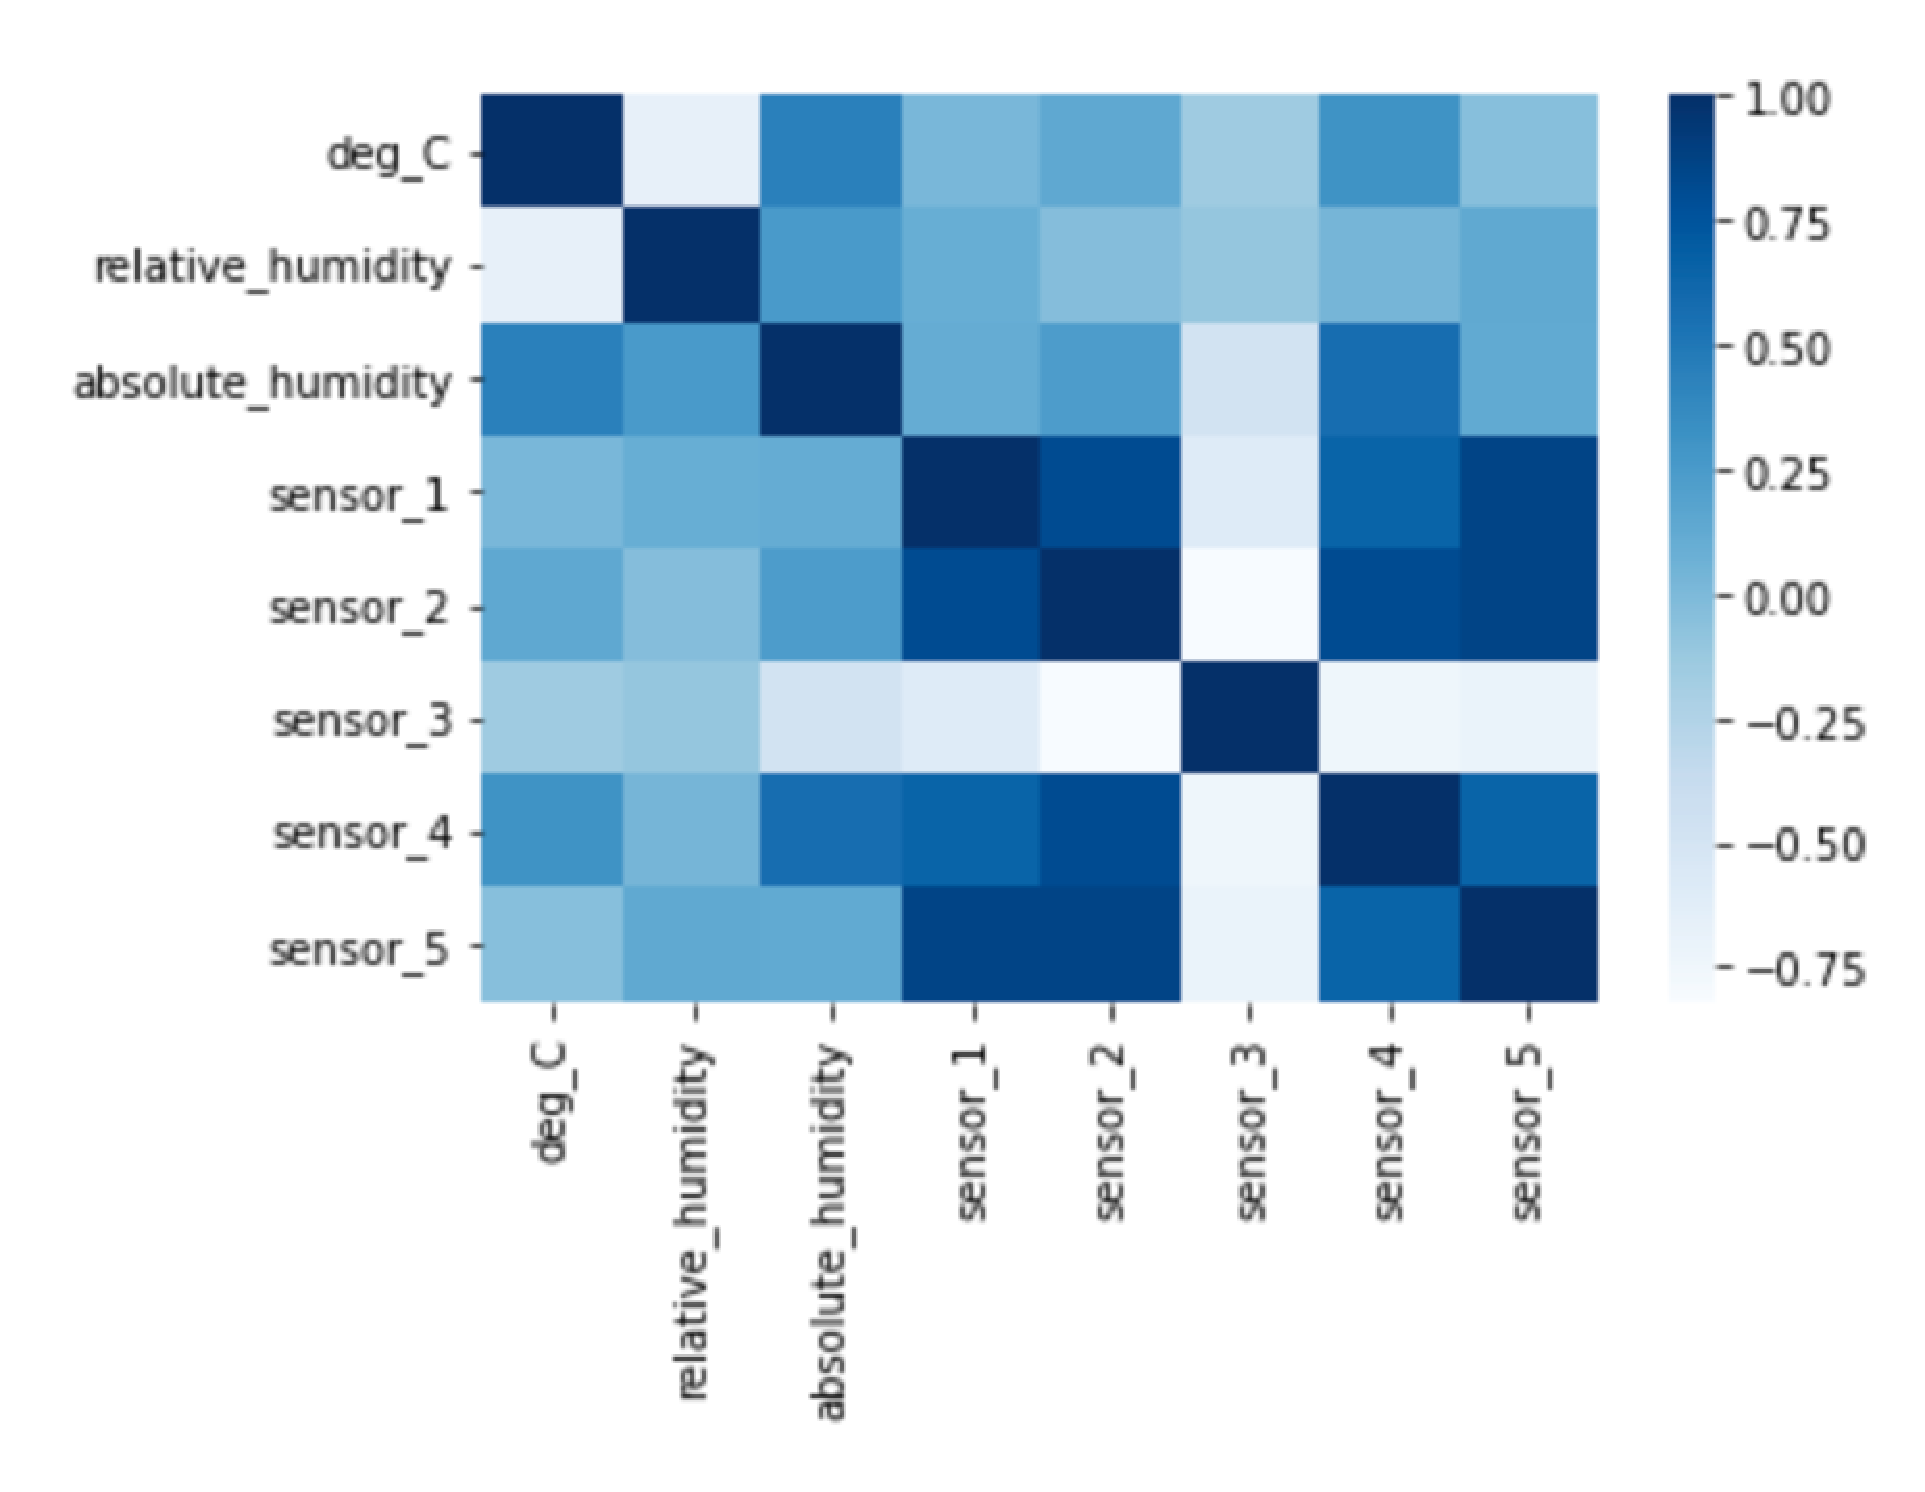
\includegraphics[width=1.0\linewidth,height=0.8\linewidth]{graphics//Fig_heatmap.eps}
  \caption{Heatmap} \label{Heatmap}
\end{figure}


Prepossessing is the initial step in machine learning approaches.
Because, all the models are driven on the existing training data. 
Therefore, training data must be clear enough having less noise.
There are so many methods to clean the data such as min-max scaling,
standard scaling and remove duplication.
Apart from that, we need to maintain data consistency among the learning process.
In this study we use, standard scaler which is available in sklearn package in python.
Then convert all the data into one consistent data format.
Further, we remove the duplicates and 
make the data more narrow by which allow to maintain clarity of data.
We maintain only relevant data items throughout the training process 
by eliminating other irrelevant data such as target variables and date time data.
Further, we analyse the data distribution 
by generating boxplot visualization as in Figure \cref{Fig_boxplot}.
This uses to identify the symmetric 
and skewness of target data in the training set before we develop the model.
Multicollinearity is a aspect which 
occurs when two or more predictor variables are correlated~\cite{uyanik2013study}. 
As a consequent, coefficients error may increase \cite{uyanik2013study}.
Then the each variables behave insignificantly, 
thought they should be significant. 
So that, the models are badly impacted 
if such model does not address this multicollinearity in an proper way.
The reasons for multicollinearity are using different 
types of variables inaccurately,
poor or null hypothesis, bad selection of a dependent variable, 
repetitions in variable, and 
a high correlation between variables and 
choice of dummy variables~\cite{farrar1967multicollinearity}.
There are certain set of solutions to 
hinder the impact of multicollinearity in linear regression.
They are obtaining more set of predictors, removing 
unwanted variables, deciding accurate independent variable 
and use rigid regression method or partial squares regression~\cite{farrar1967multicollinearity}.
Sometimes, if all these solutions may not applicable.
And then researchers decide do nothing.
For example, in this study, 
we recognize the given training data has multicollinearity due to multi 
correlations among predictors [Temperature, absolute humidity, relative humidity, sensor data] 
as depicted in Figure \ref{Fig_heatmap} and Figure \ref{Fig_Predictor_correlation}.
As a solution, we decide to implement rigid regression method 
to derive our proposed method.


\subsection{Usage of Rigid Regression}

Linear regression is most widely use learning predictive model 
which presents relationship as a straight line.
In this approach show correlation between two variables.
That means there should be one predictor for response variable/variables at a time.
Moreover, the dependent variable, which is called 
response should be continuous and independent 
variable(s) (predictor variables) can be continuous or discrete. 
In contrast, rigid regression is a technique used 
to implement multicollinearity of predictor variables 
which are highly correlated each other \cite{dong2016moving}.
Generally, rigid regression is same like 
linear regression unless it add penalty values 
to reduce the loss or error of linear regression.
This error can  be happen due to bias and/or variance of the variables.

\subsection{Efficiency Analysis}
We uses coefficient of determination to measure the performance of the proposed models. 
The coefficient of determination interprets 
how well the regression model fits testing data observations.
Further, it describes how much variation 
can be expected in the dependent/response variable.

\section{Experiment and Analysis} \label{sec-experiment}

\begin{figure}
  \selectcolormodel{rgb}
  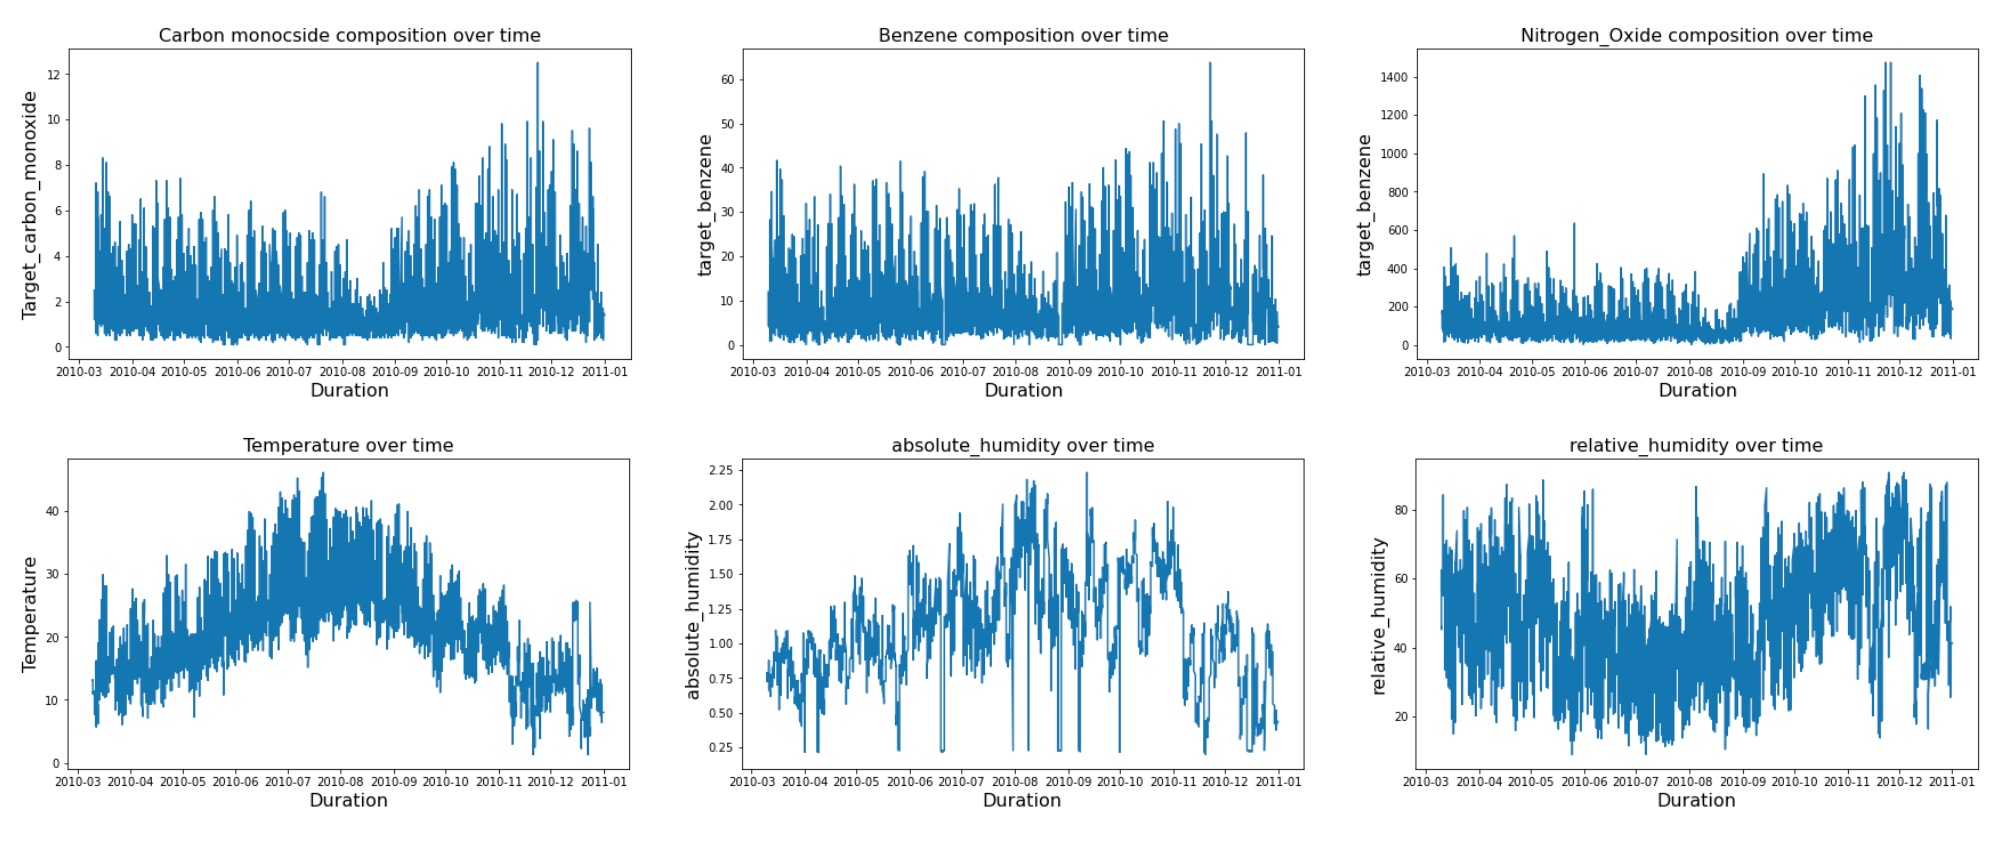
\includegraphics[width=0.9\linewidth,height=0.5\linewidth]{graphics//Fig_Correlations.eps}
  \caption{Impact of Air pollution and behavior of each pollution
  components over time. From left top corner to right top corner
  shows behavior of carbon monoxide, benzene and nitrous oxide
  respectively. From left bottom corner to right bottom corner shows
  how temperature, absolute humidity and relative humidity change
  over time} \label{Fig_Predictor_correlation}
\end{figure}


In this study we propose a model to 
predict air pollution component behavior by using rigid regression. 
We use rigid regression instead of linear regression,
to hinder the multicollinearity issue. 
As illustrated in Figure \ref{Fig_Impact} first we 
demonstrate given air pollution components behavior over time.
the given duration starts from march 2010 to January 2011.
As in Figure \ref{Fig_Impact} first row shows how each 
air particles behave over this time series. 
Based on that, we can see all three types of air shows 
high amount of concentration within September 2010 to January 2011.
And further, if we consider temperature, it seems high variance within mid of the year.
Moreover, humidity perform very fluctuation behavior over this period.
We test our proposed model using test dataset which 
includes same set of predictor variables.
The results are given in Figures \ref{Fig_Predcarbon monoxide}, \ref{Fig_Predbenzene}, \ref{Fig_Prednitrousoxide}.
Accordingly, test data prediction given in above 
figures shows that test accuracy of our model. 
Because, the test data histogram is properly fitted with test histogram.
Further, in Table \ref{tbl:overall-experiments} shows how bias and variance relates with 
different models which are separately derived to 
predict compositions of carbon monoxide, benzene and nitrous oxide.
Accordingly, it shows high bias and low variance which is common in all three models.
This indicates underfitting behavior of data points.
However, we use coefficient determination factor to 
show how well our proposed models fits the observed data. 
As mentioned in Table \ref{tbl:overall-experiments}, 
all three models has overall best performance efficiency. 
For example, carbon monoxide prediction model hold 0.82 (82\%) coefficient determination, which indicates high efficiency of the model.
And such, benzene model holds 0.95 (95\%) coefficient determination, which indicates highest efficiency.
Moreover, compare to the other two models, the model for nitrous oxide has less efficiency since it has 0.6 coefficient determination. 
This is clearly shown in Figure \ref{Fig_Prednitrousoxide} in which fits the testing histogram with training histogram.

\begin{figure}
  \centering
  \selectcolormodel{rgb}
 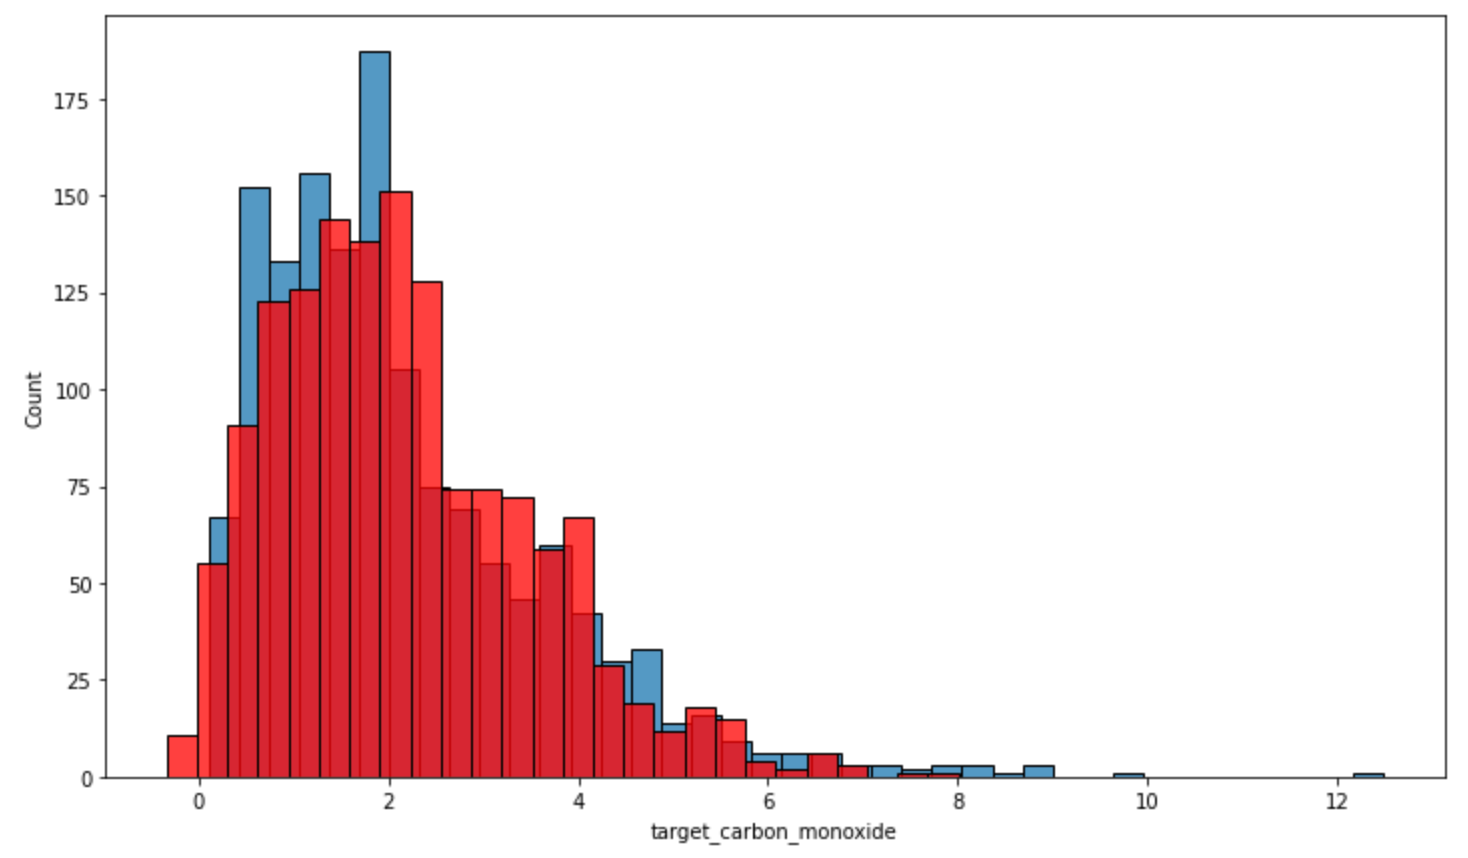
\includegraphics[width=1.0\linewidth,height=0.8\linewidth]{graphics//Fig_CM_ModelAccuracy.eps}
  \caption{Prediction accuracy for carbon monoxide results [Train-
  ing histogram indicates in blue color whereas testing histogram
  show in red color} \label{Fig_Predcarbon monoxide}
\end{figure}

\begin{figure}
  \centering
  \selectcolormodel{rgb}
 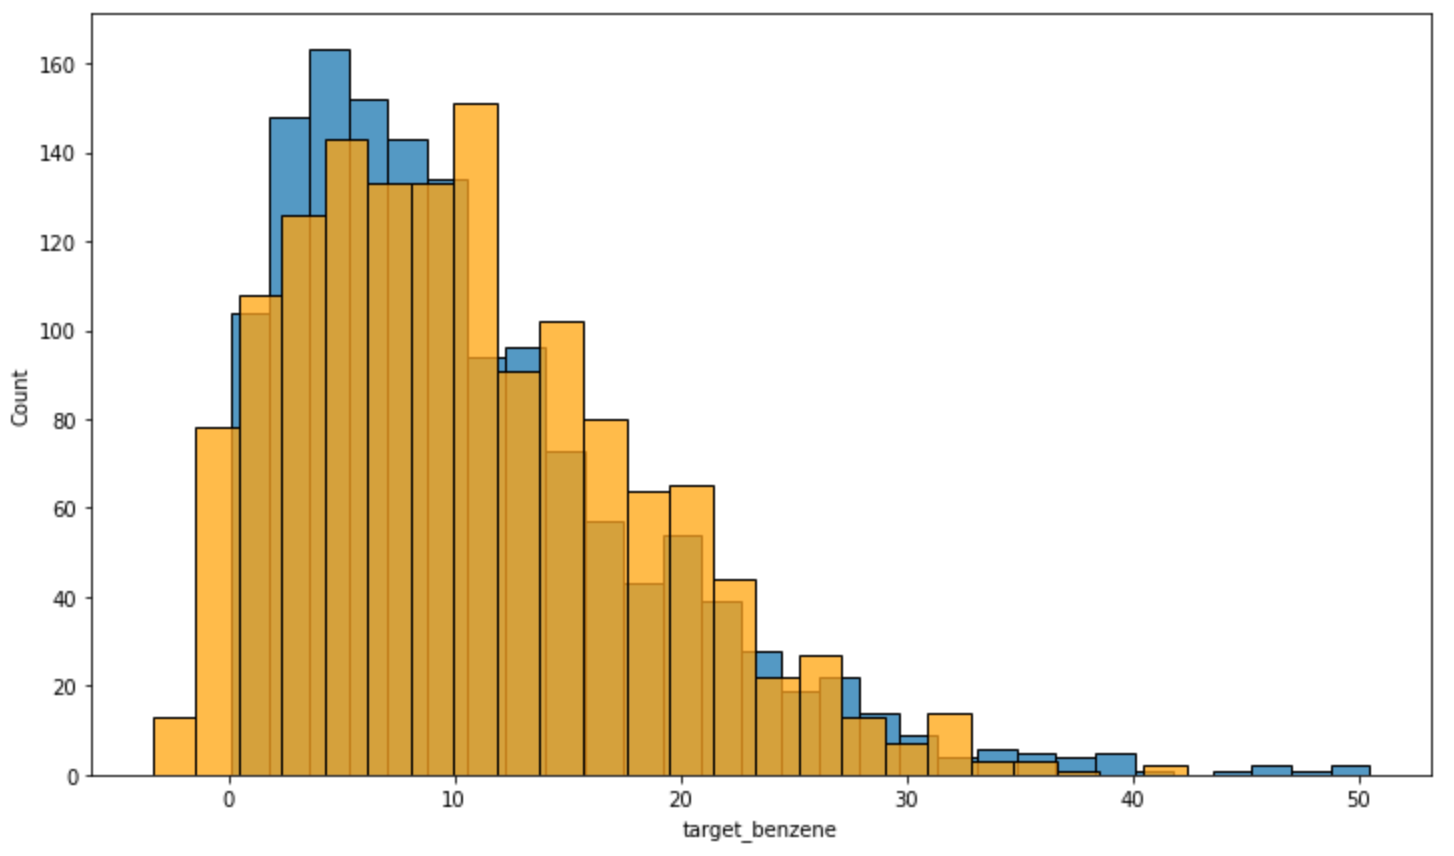
\includegraphics[width=1.0\linewidth,height=0.8\linewidth]{graphics//Fig_BenzeneModelBehavior.eps}
  \caption{Prediction accuracy for benzene results [Training his-
  togram indicates in blue color whereas testing histogram show in
  red color} \label{Fig_Predbenzene}
\end{figure}

\begin{figure}
  \centering
  \selectcolormodel{rgb}
 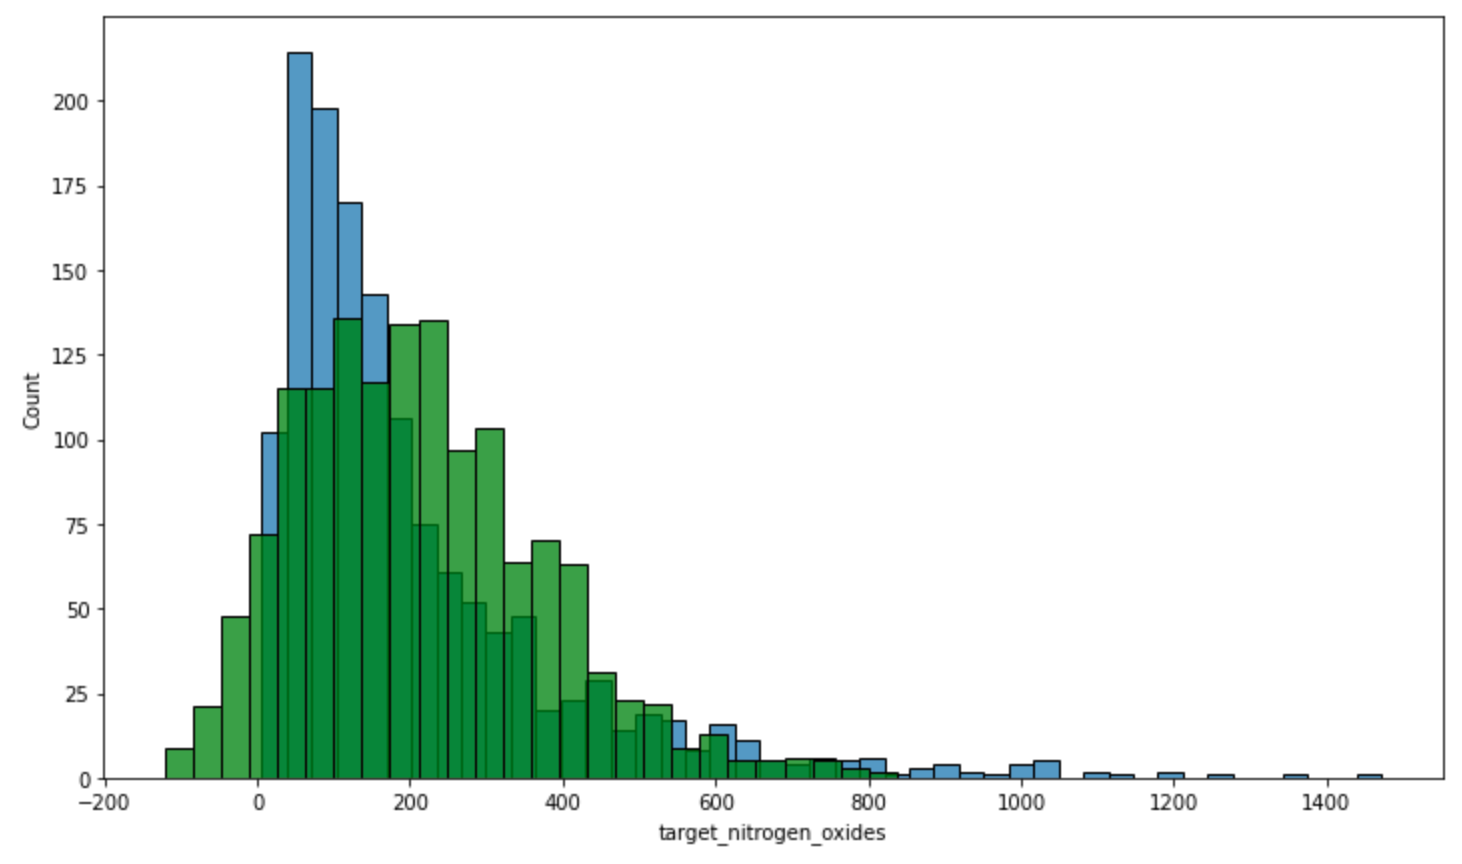
\includegraphics[width=1.0\linewidth,height=0.8\linewidth]{graphics//Fig_NOxModelBehavior.eps}
  \caption{Prediction accuracy for nitrous oxide results. [Training
  histogram indicates in blue color whereas testing histogram show
  in red color]} \label{Fig_Prednitrousoxide}
\end{figure}

\begin{table}  \centering
  \caption{Precision Comparison on Event Detection Methods}
  \label{tbl:overall-experiments}
  \begin{tabular}{cccc}
\toprule
    % after \\: \hline or \cline{col1-col2} \cline{col3-col4} ...
    & CM & Benzene &NO \\
\midrule
Bias & 0.38 & 3.379 & 12916.6 \\
Variance & 0.001 & 0.009 & 30.591 \\
CD Training & 0.82 & 0.95 & 0.68 \\
CD Testing & 0.83 & 0.94 & 0.66 \\
\bottomrule
\end{tabular}
\end{table}


\section{Conclusions} \label{sec-conclusions}

In this study we propose prediction model to predict air pollution components which are specified as carbon monoxide, benzene and nitrous oxide. We uses multiple predictors such as temperature, absolute and relative humidity and five sensor data.
We identify that these predictors are correlated among each other.
Therefore, we reveals the need of handling multicollinearity in this study.
Consequently, we use rigid linear regression instead general linear regression method.
We clearly show the performance efficiency of proposed 
models using determination of coefficient, bias and variance scores for each models.
We recommend to expand this study to evaluate how well these prediction models behave on dding more noisy data.
This may help to increase the prediction accuracy.
Further, we suggest to implement this study to increase the amount of predictors to predict air pollution.

\section*{Acknowledgement}
I would acknowledge to all the people who helped me to success this effort. Specifically I would thank for the directors and all the members in flip00 for directing me towards this projects.


